\documentclass[11pt, a4paper, twoside]{article}   	% use "amsart" instead of "article" for AMSLaTeX format

\usepackage{geometry}                		% See geometry.pdf to learn the layout options. There are lots.
\usepackage{pdfpages}
\usepackage{caption}
\usepackage{minted}
\usepackage[german]{babel}			% this end the next are needed for german umlaute
\usepackage[utf8]{inputenc}
\usepackage{color}
\usepackage{graphicx}
\usepackage{titlesec}
\usepackage{fancyhdr}
\usepackage{lastpage}
\usepackage{hyperref}
\usepackage[autostyle=false, style=english]{csquotes}
\usepackage{mathtools}
\usepackage{tabularx}
% http://www.artofproblemsolving.com/wiki/index.php/LaTeX:Symbols#Operators
% =============================================
% Layout & Colors
% =============================================
\geometry{
   a4paper,
   total={210mm,297mm},
   left=20mm,
   right=20mm,
   top=20mm,
   bottom=30mm
 }	

\definecolor{myred}{rgb}{0.8,0,0}
\definecolor{mygreen}{rgb}{0,0.6,0}
\definecolor{mygray}{rgb}{0.5,0.5,0.5}
\definecolor{mymauve}{rgb}{0.58,0,0.82}

\setcounter{secnumdepth}{4}


% the default java directory structure and the main packages
\newcommand{\srcDir}{/src/main/java}
% =============================================
% Code Settings
% =============================================
\newenvironment{code}{\captionsetup{type=listing}}{}
\newmintedfile[cppSourceFile]{cpp}{
	linenos=true, 
	frame=single, 
	breaklines=true, 
	tabsize=2,
	numbersep=5pt,
	xleftmargin=10pt,
	baselinestretch=1,
	fontsize=\footnotesize
}
\newmintinline[inlineCpp]{cpp}{}
\newminted[cppSource]{cpp}{
	breaklines=true, 
	tabsize=2,
	autogobble=true,
	breakautoindent=false
}
% =============================================
% Page Style, Footers & Headers, Title
% =============================================
\title{Übung 1}
\author{Thomas Herzog}

\lhead{Übung 1}
\chead{}
\rhead{
\includegraphics[scale=0.10]{FHO_Logo_Students.jpg}}

\lfoot{S1610454013}
\cfoot{}
\rfoot{ \thepage / \pageref{LastPage} }
\renewcommand{\footrulewidth}{0.4pt}
% =============================================
% D O C U M E N T     C O N T E N T
% =============================================
\pagestyle{fancy}
\begin{document}
\setlength{\headheight}{15mm}
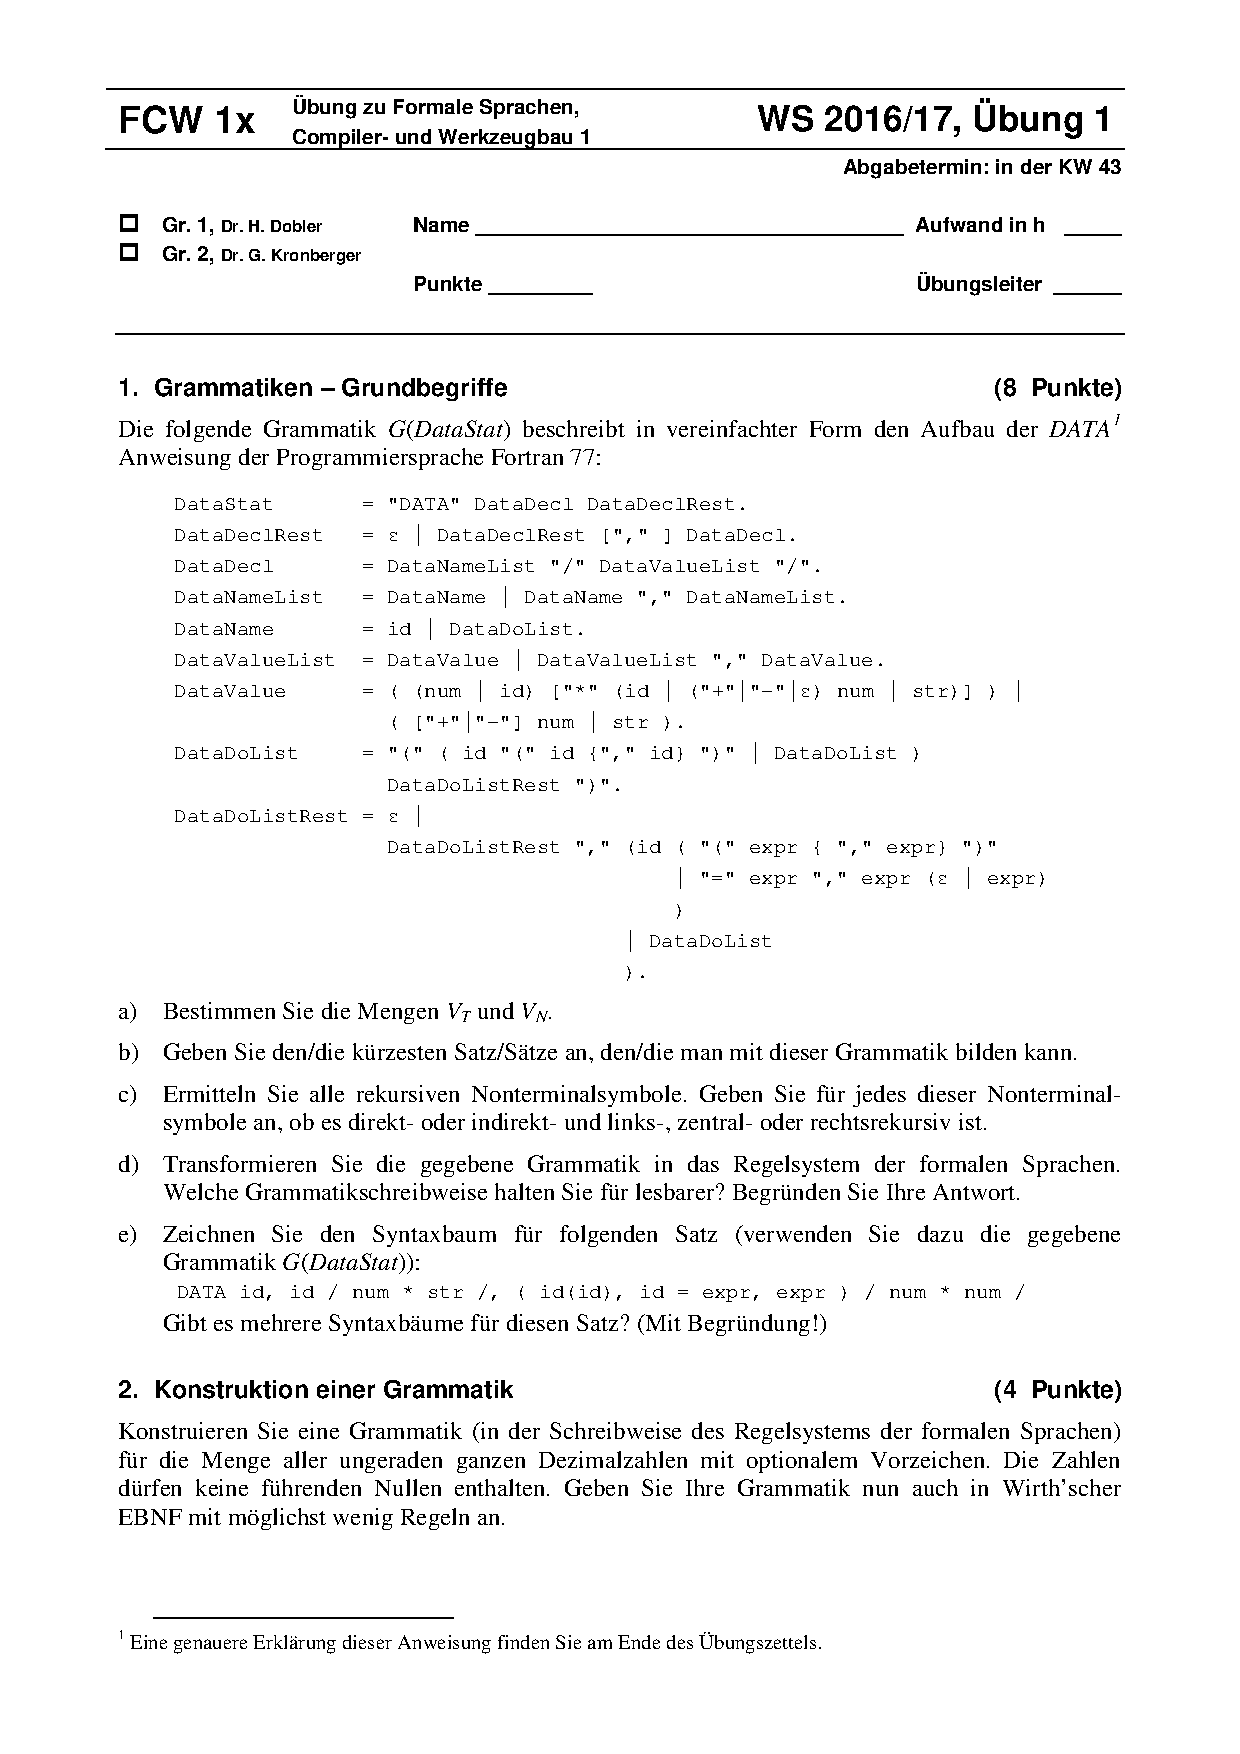
\includepdf[pages={1,2}]{Fcw1x01A.pdf}

% Section gramar and basics 
\section {Grammatiken - Grundbegriffe}
Dieser Teil der Dokumentation behandelt die Aufgabe 1 der ersten Übung.
\subsection{Die Mengen $V_{T}$ und $V_{N}$}
$V_{N}=\{$ DataStat, DataDeclRest, DataDecl, DataNameList, DataName, DataValueList, DataValue, DataDoList, DataDoListRest $\}$
\newline
\newline
Alle Nichtterminalsymbole befinden sich links in der Grammatik, wobei das Nichtterminalsymbol \emph{DataStat} das Satzsymbol ist.
\newline
\newline
\newline
$V_{T}=\{$ \enquote{Data},\enquote{,}, \enquote{/}, \enquote{(}, \enquote{)},\enquote{=}, \enquote{*}, \enquote{+}, \enquote{-}, \enquote{=}, expr, id, num, str $\}$
\newline
\newline
Alle Terminalsymbole kommen nicht auf der linken Seite der Grammatik vor und können nicht weiter abgeleitet werden. Das Symbol \enquote{$\epsilon$} ist ein Metasymbol, dass die leere Kette repräsentiert und ist weder ein Nichtterminalsymbol oder ein Terminalsymbol.
\newline
\newline
\newline
$V=V_{T} \cup V_{N}$
\newline
\newline
Die Menge $V$ ist das Alphabet der Grammatik und ist die Vereinigung der Menge der Nichtterminalsymbole und der Menge der Terminalsymbole. Da das Symbol $\epsilon$ ein Metasymbol ist, ist es nicht Teil der Grammatik und auch kein Teil des Alphabets der Grammatik.

\subsection{Kürzeste Sätze der Grammatik}
DataStat $\xRightarrow{L}$ \enquote{DATA} \underline{DataDecl} DataDeclRest
\newline
\null\hspace{1.55cm} $\xRightarrow{L}$ \enquote{DATA} \underline{DataNameList} \enquote{/} DataValueList \enquote{/} DataDeclRest
\newline
\null\hspace{1.55cm} $\xRightarrow{L}$ \enquote{DATA} \underline{DataName} \enquote{/} DataValueList \enquote{/} DataDeclRest
\newline
\null\hspace{1.55cm} $\xRightarrow{L}$ \enquote{DATA} id \enquote{/} \underline{DataValueList} \enquote{/} DataDeclRest
\newline
\null\hspace{1.55cm} $\xRightarrow{L}$ \enquote{DATA} id \enquote{/} \underline{DataValue} \enquote{/} DataDeclRest
\newline
\null\hspace{1.55cm} $\xRightarrow{L}$ \enquote{DATA} id \enquote{/} num  \enquote{/} DataDeclRest
\newline
\null\hspace{1.55cm} $\xRightarrow{L}$ \enquote{DATA} id \enquote{/} num  \enquote{/}
\newline
\newline
\newline
%
DataStat $\xRightarrow{L}$ \enquote{DATA} \underline{DataDecl} DataDeclRest
\newline
\null\hspace{1.55cm} $\xRightarrow{L}$ \enquote{DATA} \underline{DataNameList} \enquote{/} DataValueList \enquote{/} DataDeclRest
\newline
\null\hspace{1.55cm} $\xRightarrow{L}$ \enquote{DATA} \underline{DataName} \enquote{/} DataValueList \enquote{/} DataDeclRest
\newline
\null\hspace{1.55cm} $\xRightarrow{L}$ \enquote{DATA} id \enquote{/} \underline{DataValueList} \enquote{/} DataDeclRest
\newline
\null\hspace{1.55cm} $\xRightarrow{L}$ \enquote{DATA} id \enquote{/} \underline{DataValue} \enquote{/} DataDeclRest
\newline
\null\hspace{1.55cm} $\xRightarrow{L}$ \enquote{DATA} id \enquote{/} id  \enquote{/} DataDeclRest
\newline
\null\hspace{1.55cm} $\xRightarrow{L}$ \enquote{DATA} id \enquote{/} id  \enquote{/}
\newpage

\parindent0pt DataStat $\xRightarrow{L}$ \enquote{DATA} \underline{DataDecl} DataDeclRest
\newline
\null\hspace{1.55cm} $\xRightarrow{L}$ \enquote{DATA} \underline{DataNameList} \enquote{/} DataValueList \enquote{/} DataDeclRest
\newline
\null\hspace{1.55cm} $\xRightarrow{L}$ \enquote{DATA} \underline{DataName} \enquote{/} DataValueList \enquote{/} DataDeclRest
\newline
\null\hspace{1.55cm} $\xRightarrow{L}$ \enquote{DATA} id \enquote{/} \underline{DataValueList} \enquote{/} DataDeclRest
\newline
\null\hspace{1.55cm} $\xRightarrow{L}$ \enquote{DATA} id \enquote{/} \underline{DataValue} \enquote{/} DataDeclRest
\newline
\null\hspace{1.55cm} $\xRightarrow{L}$ \enquote{DATA} id \enquote{/} str  \enquote{/} DataDeclRest
\newline
\null\hspace{1.55cm} $\xRightarrow{L}$ \enquote{DATA} id \enquote{/} str  \enquote{/}
\newline
\newline
Das Nichtterminalsymbol \emph{DataValue} kann in drei Varianten abgeleitet werden, \emph{id}, \emph{num} und \emph{str}. 

\subsection{Rekursionen der Nichtterminalsymbole}
    \begin{tabularx}{\textwidth}{|>{\centering}X|>{\centering}X|>{\centering\arraybackslash}X|}
    \hline
    \textbf{Nichtterminalsymbol} & \textbf{direkt/indirekt rek.} & \textbf{links/rechts rek.} \\ \hline
    DataDeclRest                 &           direkt rek.         &           links rek.\\ \hline
    DataDecl                     &                               & \\ \hline
    DataNameList                 &           direkt rek.         &           rechts rek. \\ \hline
    DataName                     &                               & \\ \hline
    DataValueList                &           direkt rek.         &           links rek. \\ \hline
    DataValue                    &                               & \\ \hline
    DataDoList                   &                               & \\ \hline
    DataDoListRest               &                               & \\ \hline
    \end{tabularx}

%\subsubsection{MainFX.java}
%Diese Klasse stellt die Main Klasse für die JavaFX Applikation dar.
%\begin{code}
%	\caption{MainFX.java}
%	\javaSourceFile{\fxSource/main/MainFX.java}
%\end{code}
\end{document}